
\documentclass{beamer}

\usepackage{graphicx}
\usepackage{tikz}
\usetikzlibrary{positioning}
% \usepackage[mode=buildnew]{standalone} % Allows inclusion of standalone files

\usepackage{caption}
\usepackage{subcaption}

% define a style for a tikz node with a smaller font size and texttt font
\tikzset{message/.style={font=\small\ttfamily}}

\usetheme{default} % Change "default" to a specific theme, e.g., "Madrid" or "Berlin"
\title{ORCA: Observability with Realtime Control and Aggregation}
\author[Left Text]{Ankush Jain}
\institute{CMU}
\date{\today}

\begin{document}

% \begin{frame}
%   \titlepage % Generates the title slide
% \end{frame}

\begin{frame}{Agenda 20250211: Overlay code walkthrough}
	\begin{enumerate}
		\item Addressing, bootstrapping
		\item Mercury, progress
		\item Topologies
		\item Logging, options
	\end{enumerate}
\end{frame}

\begin{frame}{Testing Topologies}
	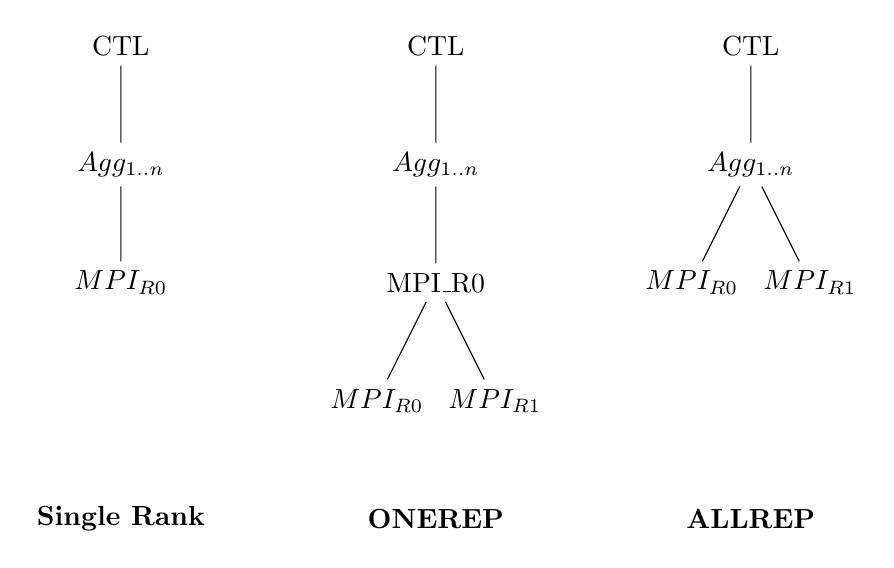
\begin{tikzpicture}
		% shift scope by 1cm xshift
		\begin{scope}[xshift=1cm]
			\node (a) {CTL}
			child { node (b) {$Agg_{1..n}$}
					child { node (c) {$MPI_{R0}$} }
				};
			\node at (0, -6) {\textbf{Single Rank}};
		\end{scope}

		\begin{scope}[xshift=5cm]
			\node (a) {CTL}
			child { node (b) {$Agg_{1..n}$}
					child {
							node (c) {MPI\_R0}  {
									child { node (d) {$MPI_{R0}$} }
									child { node (e) {$MPI_{R1}$} }
								}
						}
				};
			% add a text node LABEL at the bottom
			\node at (0, -6) {\textbf{ONEREP}};
		\end{scope}

		\begin{scope}[xshift=9cm]
			\node (a) {CTL} {
				child { node (b) {$Agg_{1..n}$}
						child { node (c) {$MPI_{R0}$} }
						child { node (d) {$MPI_{R1}$} }
					}
			};
			% add a text node LABEL at the bottom
			\node at (0, -6) {\textbf{ALLREP}};
		\end{scope}

	\end{tikzpicture}
\end{frame}

% -- SEQ DIAG --
% \begin{frame}
% 	\begin{tikzpicture}[node distance=2cm]
%
% 		% Entities
% 		\node (MPI) [draw, rectangle] {MPI};
% 		\node (CTL) [right=4cm of MPI, draw, rectangle] {CTL};
% 		\node (AGG) [right=4cm of CTL, draw, rectangle] {AGG};
%
% 		% Messages
% 		\draw[->] (MPI) -- node[above] {Hello} (CTL);
% 		\draw[<-] (MPI) -- node[below] {Hello Back} (CTL);
%
% 		\draw[->] (MPI) -- node[above] {Hello} (AGG);
% 		\draw[<-] (MPI) -- node[below] {Hello Back} (AGG);
%
% 	\end{tikzpicture}
% \end{frame}
% -- SEQ DIAG --

\begin{frame}{Sequence Diagram - TCP Discovery}
	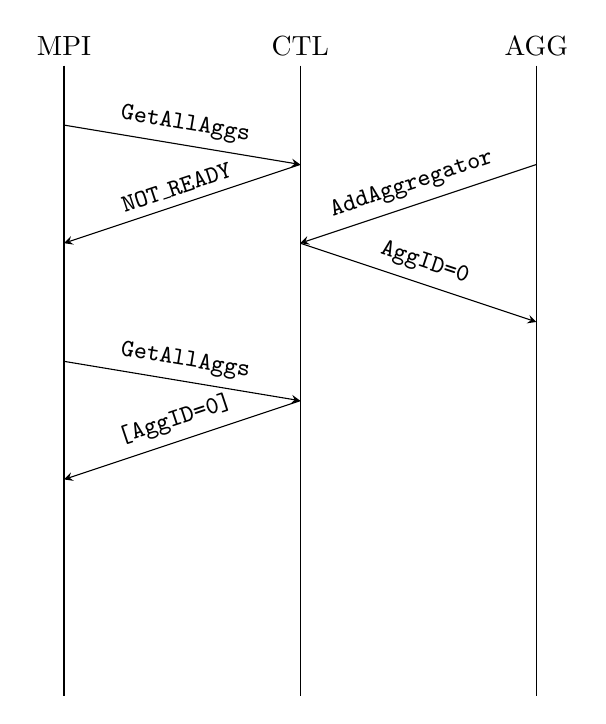
\begin{tikzpicture}[>=stealth]

		% Entities and threads
		\node (MPI) at (0, 0) {MPI};
		\draw (MPI.south) -- ++(0, -8) coordinate (MPI-thread);

		\node (CTL) at (3, 0) {CTL};
		\draw (CTL.south) -- ++(0, -8) coordinate (CTL-thread);

		\node (AGG) at (6, 0) {AGG};
		\draw (AGG.south) -- ++(0, -8) coordinate (AGG-thread);

		% Messages
		\draw[->] (0, -1) -- (3, -1.5) 
      node[message, midway, above, sloped] {GetAllAggs};
		\draw[->] (3, -1.5) -- (0, -2.5) 
      node[message, midway, above, sloped] {NOT\_READY};

		\draw[->] (6, -1.5) -- (3,-2.5) 
      node[message, midway, above, sloped] {AddAggregator};
		\draw[->] (3, -2.5) -- (6,-3.5) 
      node[message, midway, above, sloped] {AggID=0};

		\draw[->] (0, -4) -- (3, -4.5) 
      node[message, midway, above, sloped] {GetAllAggs};
		\draw[->] (3, -4.5) -- (0, -5.5) 
      node[message, midway, above, sloped] {[AggID=0]};

	\end{tikzpicture}
\end{frame}

\begin{frame}{Overlay Overview}
	\begin{itemize}
		\item Wrapper over Mercury, route map, addresses, progress
		\item Will discover MPI topology and exchange routes
		\item Will not discover CTL/AGG topology
		\item (These rely on TCP discovery protocol, hence external)
	\end{itemize}
\end{frame}

\begin{frame}{Overlay Implementation}

	\begin{itemize}
		\item All entities are addressed using an \texttt{ovid\_t} (wrapper over int)
		      \begin{itemize}
			      \item For MPI ranks, \texttt{ovid\_t} is the rank itself
			      \item CTL has a reserved ovid.
			      \item AGGs ovid is \texttt{(1 << 24) || agg\_id}.
		      \end{itemize}
		\item \texttt{SendMessage(Envelope env)}: triggers an RPC
		\item \texttt{EnqueueAddrs(string hg\_addr, bool lookup)}
		      \begin{itemize}
            \item Enqueues addrs received during initialization
			      \item If lookup is true, will trigger \texttt{HG\_Addr\_lookup}
			      \item Otherwise need to call \texttt{LookupQueuedAddresses} after
            \item (Should not trigger lookups in message handlers)
            \item (No common delivery thread for now)
		      \end{itemize}
	\end{itemize}

\end{frame}

\begin{frame}{Mercury Overview}
	\begin{itemize}
		\item Currently hardcoded Mercury params (shm etc), TODO
		\item Have a simple progress loop for now
		\item Assuming one address per \texttt{ovid\_t}
		\item (Mercury will automatically use \texttt{na+sm} for local comm AFAIK)
	\end{itemize}
\end{frame}

\begin{frame}{Misc}
	\begin{itemize}
		\item Logging: using Chuck's mlog, may need setup tweaks
		\item Options: common options handling for MPI/CTL/AGG
		      \begin{itemize}
			      \item common shared struct, use what you need
			      \item Priority 1: config file
			      \item Priority 2: env var
			      \item Priority 3: default
			      \item No CLI params
		      \end{itemize}
	\end{itemize}
\end{frame}

\begin{frame}{Extending ORCA}
	\begin{itemize}
		\item Idea: implement "apps" on top, separate from core
		\item Carve out your own top-level XDR op
		\item Implement your app as separate modules
		\item Add objects to MPI/CTL/AGG classes and link handlers
	\end{itemize}
\end{frame}

\begin{frame}{Artifacts For Now}
	\begin{itemize}
		\item CTL/AGG/MPIRank - basic executables with hardcoded params
		\item MPITopo: "integration test"
		\item Some other tests
	\end{itemize}
\end{frame}

\begin{frame}{Next Steps}
	\begin{itemize}
		\item Complete remaining overlay bits: gluing topology, forwarding, broadcast etc.
		\item Add an on-overlay key-value cache
		      \begin{itemize}
			      \item Idea: tree node triggers a lookup at parent
			      \item Parent responds if a cache hit
			      \item If not, parent forwards to AGG
			      \item Multiple lookups get coalesced
			      \item Will be used at least for Probe ID assignment
		      \end{itemize}
		\item Switch to datafusion/Rust query planning
		\item Some CTL logic is a todo. Do it concurrently or after SQL.

	\end{itemize}
\end{frame}

\end{document}
